\newpage


\section{Введение}
Анализ физической активности человека производится при помощи мобильных телефонов, разумных часов~\cite{kwapisz2010, wang2014}. 
Эти устройства используют акселерометр, гироскоп и магнитометр. 
Цель данной работы заключается в  разметке и распознавании человеческой активности~\cite{Ignatov2015, Olivares2012, cinar2018}, а также поиска начала каждого действия~\cite{motrenko2015}. 
Примерами одного сегмента действия служит шаг, шаг бега, приседание, прыжок и др. 
Исследуются последовательности, которые состоят не менее чем из двух подряд идущих сегментов, которые соответствуют одному и тому жу типу человеческой активности.

\begin{figure}[h!t]\center
\subfloat[]
{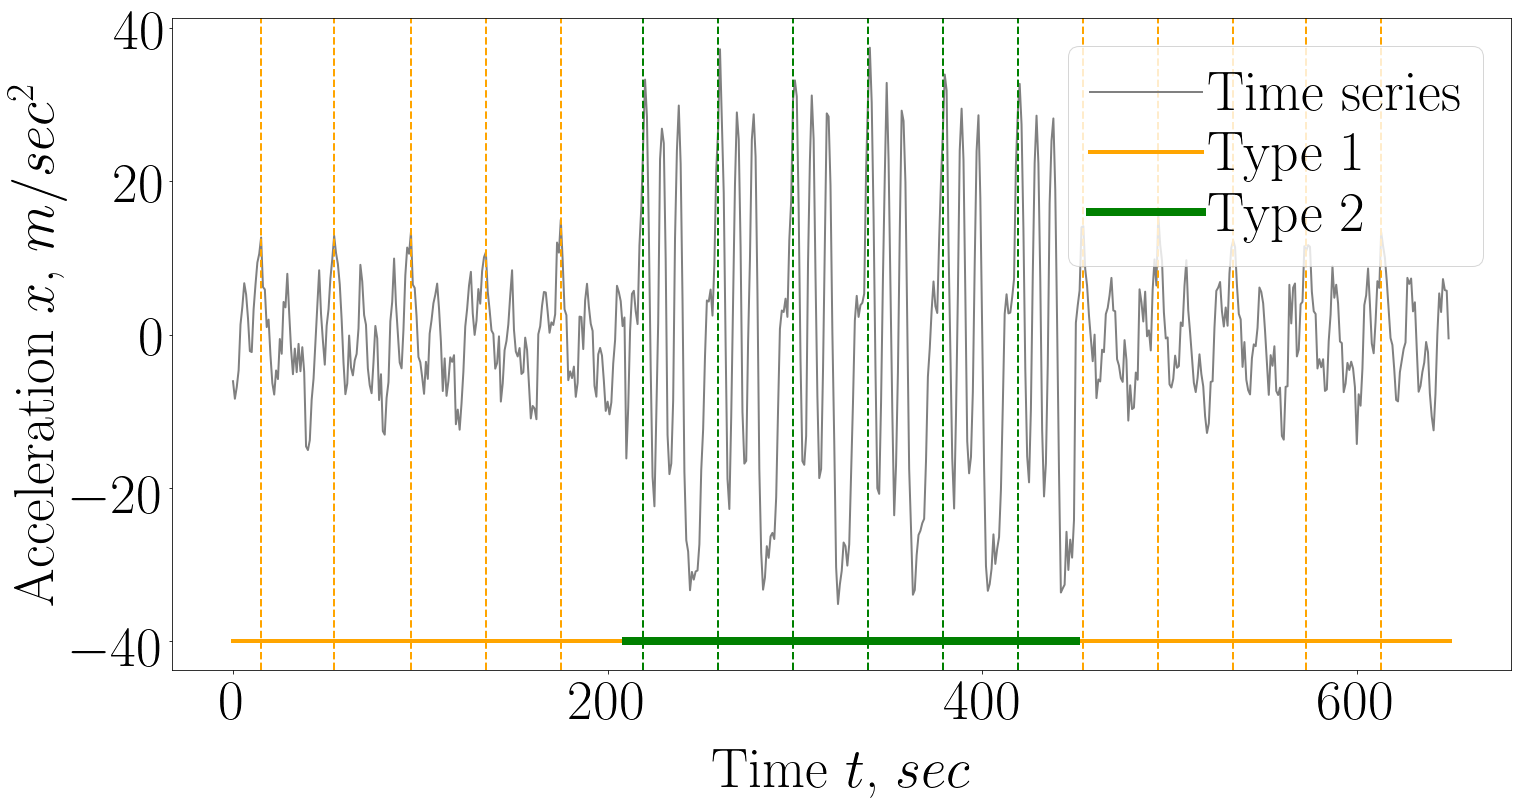
\includegraphics[width=0.5\textwidth]{results/example}\label{example:1}}
\subfloat[]
{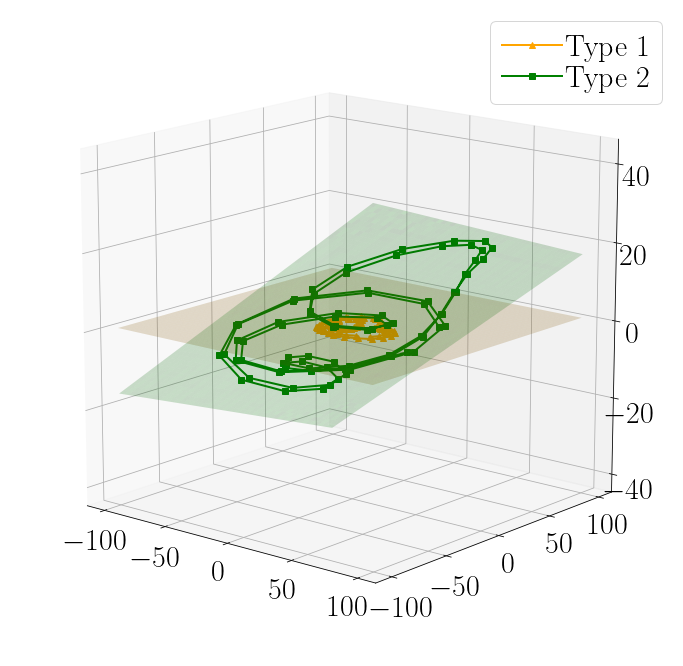
\includegraphics[width=0.5\textwidth]{results/example_phase}\label{example:2}}\\
\caption{Временной ряд, с разметкой на кластеры: a) временной ряд с ассесорской разметкой на кластеры и выделением начала квазипериодического сегмента; b) проекция фазовых траекторий на первые две главные компоненты }
\end{figure}

Временные ряды~---~это объекты сложной структуры. 
При их классификации значимую роль играет модель построения признакового пространства.
В данной работе объектом анализа и кластеризации является точка на оси времени. 
Решается задача кластеризации точек временного ряда. 
При \textit{кластеризации} каждой точке временного ряда ставится в соответствие метка из конечного множества меток. 
Каждая метка соответствует одному характерному физическому действию. \textit{Сегмент} это часть временного ряда, которая соответствует одному характерному физическому действию, например: шаг двумя ногами при ходьбе, или шаг двумя ногами при беге.
Последовательность сегментов, которые соответствуют одному физическому действия образуют \textit{цепочку} действий. 
Предполагается, что цепочка действий образует квазипериодическую последовательность значений временного ряда.
Последовательность точек $\{b_t\}_{t=1}^{N}$ назовем \textit{квазипериодической} с периодом $T$, если для всех $t$ найдется $\Delta$, такое что:
\begin{equation}
\label{eq:int:1}
\begin{aligned}
b_t \approx b_{t+T+\Delta}, \quad \left|\Delta\right| \ll T.
\end{aligned}
\end{equation}
Пример кластеризации и разбиения ряда на сегменты показан на рис.~\ref{example:1}. Данный ряд разбит на два характерных физических действия, которые обозначаются Type~1 и Type~2. Также данный ряд содержит в себе две квазипериодические цепочки действий.

Решение задачи кластеризации состоит из двух этапов. 
Во-первых, для получения признакового описания временного ряда предлагается алгоритм локальной аппроксимации временного ряда при помощи метода главных компонент~\cite{Shiglavsi1997}. 
Под \textit{локальной} аппроксимацией временного ряда подразумевается, что для признакового описания его точки используется не весь ряд, а только некоторая окрестность данной точки. 
В качестве признакового описания точки временного ряда рассматриваются две главные компоненты \textit{сегмента фазовой траектории} в окрестности данной точки.
На рис.~\ref{example:2} показаны две первые главные компоненты \textit{фазовых траекторий}, а также проекция фазовых траекторий на эти компоненты.
Они соответствуют разным физическим действиям, которые обозначаются Type~1 и Type~2, внутри одного временного ряда.
Как видно плоскости, которые порождены данными главными компонентами не совпадают. 
Это говорит о том, что наблюдаются различные действия. 
Во-вторых, вводится функция расстояния в построенном пространстве признакового описания. 
Данная функция является расстояниям между двумя базисами некоторых подпространств внутри всего фазового пространства временного ряда.
На рис.~\ref{example:2} данная функция является некоторым расстояниям между двумя плоскостями.
Получив расстояния между точками временного ряда, выполним кластеризацию данных точек.
Задача сегментации внутри каждого кластера решается при помощи метода, который рассмотрен в~\cite{motrenko2015}.

Для решения задачи кластеризации точек временного ряда вводятся предположения. 
Предполагается, что периоды различных сегментов различаются незначительно, причем известны минимальный и максимальный периоды сегмента и число различных сегментов внутри временного ряда. 
Также предполагается, что тип активности во времени не меняется часто, а также что фазовые траектории разных сегментов являются различными. 

Проверка и анализ метода кластеризации проводится на синтетической и реальной выборках. 
Синтетическая выборка построенная при помощи суммы нескольких первых членов ряда Фурье со случайными коэффициентами. 
Эксперимент по сегментации временного ряда проводился на простых синусоидальных сигналах с произвольной амплитудой и частотой. 
Реальные данные получены при помощи мобильного акселерометра, который снимал показания во время некоторой физической активности человека. 

\section{Анализ литературы}
В~\cite{kwapisz2010} рассматриавется метод построения признакового описания на основе экспертно заданых порождающих функций.
В~\cite{lukashin2003} рассматривается метод построения признаков на основе гипотезы порождения данных. 
В~\cite{Ivkin2015} рассматривается комбинированное признаковое описание на основе данных методов. 
В~\cite{Katrutsa2015} рассматривается проблема построение признакового пространства и предлагается критерий избыточности выбранных признаков.

Работа~\cite{motrenko2015} является ближайшей работой по данной теме. Она заключается в поиске начала сегмента внутри квазипериодического сигнала, который состоит, только из одной цепочки действий. Этот метод основан на исследовании фазового пространства, а именно поиска устойчивой гиперплоскости, которая делит фазовое пространство на две равные части. В качестве начала сегмента выбираются точки, которые находятся близко к данной гиперплоскости. В~\cite{motrenko2015} предлагается выполнить проекцию фазового пространства на первые две главное компоненты, после чего провести устойчивую прямую, выделив начала каждого сегмента. 
Данный метод имеет недостаток в том, что позволяет находить начало только для временного ряда, который состоит из квазипериодического сигнала единственного типа.


Также близкой является работа~\cite{cinar2018}.  Данная работа заключается в поиске периодической структуры внутри ряда при помощи модели LSTM с модифицированным механизмом Attention. Предполагается, что механизм Attention будет давать максимальное значение score в точках, которые удаленны от данной на целое количество периодов.
